\documentclass{IEEEtran}
\usepackage[top=1in, right=1in, bottom=1in, left=1in]{geometry}
\usepackage{amsfonts}
\usepackage{graphicx}
\usepackage{enumerate}
\usepackage{multicol}
\usepackage{amsmath}
\usepackage{subcaption}
\usepackage{listings}
\usepackage{algpseudocode}
\usepackage{algorithm}
\usepackage{svg}

\title{Flood alert application using real time images by applying machine learning algorithms}
\author{\IEEEauthorblockN{Name, Name}\\
\IEEEauthorblockA{Dept. of Computer Science \& Technology, Indian Institute of Engineering Science \& Technology, Shibpur, Howrah, India\\
Email: anonymous1@gmail.com, anonymous2@gmail.com}}

\begin{document}
\maketitle
\begin{abstract}
In this paper, we develop an android application that provides real time updates and prompt flow of authentic information of flood ravaged areas to the public. The application would take as input the sets of images belonging to flood affected areas from rescue personnel, authenticate and filter them using deep learning approaches. The severity of floods is estimated and plotted on a map using the geolocations of the images. The data is analyzed by using clustering techniques and visualized on the map. Subsequently, the affected areas and their peripheries are discovered for immediate relief operations.
\end{abstract}
\section{Introduction}
Extreme climate changes have become the new norm. Disaster events and their scale continue to increase. Therefore, it has become imperative to devise a quick disaster response system for minimizing the magnitude of damage and reducing the casualties. The cases of flood related disasters have drastically increased especially in India with a dense population in coastal areas where the destruction due to cyclones is massive.\\
The Arabian sea is heating up leading to an increase in cyclonic activity in the area. On the east coast as well, several natural disasters have occurred of great proportions. Recent disasters such as cyclone Aila in 2009, cyclone Fani in 2019, cyclone Amphan in 2020, cyclone Nisarga in 2020, and many more have shown how man is helpless when nature’s fury has its say.\\
Other than cyclones, monsoonal floods cause mayhem as well, with commuters getting stuck in waterlogged streets, open wires electrifying nescient citizens, loss of livelihood and shelters, etc.
\subsection{Motivation}
Destruction due to floods can only be mitigated by immediate response to crises.\\
Civic volunteers and NDRF personnel (fondly called the Rescuers) are those warriors who tackle such grave situations and provide a helping hand to the victims of the afflicted. Their work and their contribution to society are unparalleled.\\
In this age of technology, if we can integrate such disaster response systems with cutting edge technology, we would be better equipped to handle crises. With the support of digital platforms, the information can be quickly communicated to disaster management teams about the severity of inundation.
\subsection{Proposed method}
The aim was to create an application that would be helpful for the smooth flow of relevant information and subsequently result in swift actions at the eventuality of a flood related disaster.\\
This application would be useful for the general public as they would be promptly notified of the flood affected zones in their respective cities and where they should not be venturing out. \\
The civic volunteers and NDRF officials would play a major role in this transfer of real time information by uploading images of the inundated localities in different pockets of the city to the flood alert application. This would facilitate citizens to be aware of the latest developments.\\
Social media images are a valuable source of information and have been used in building such disaster mitigation applications previously. However, they lack important information and are also of lesser resolution. The geolocation from the metadata of images is stripped off which makes it difficult for accurate mapping of flood affected areas. Moreover, there might be too many farce images that might be of a different location or a different date leading to inconsistencies and  delays in the hazard mitigation process.\\
The application extracts geolocation from metadata of the images instead of using the location from which the images are uploaded. This is beneficial in case there is poor internet supply in the affected areas and the civic volunteers choose to upload images from an unaffected area with better internet coverage.
\subsubsection{Authentication}
We found out that several images that are posted by news agencies or in social media do not convey any pictorial information about the said event. In flood related disasters, several images are circulated over the internet. However, only half the number of images are relevant to the event.\\
Thus, these images, once having been uploaded to the server undergo a verification process. The server checks the validity of the images as to whether it belongs to the city as has been specified by the user who has pushed the image to the server.\\
Another layer of check is done where the image is passed through a machine learning model that authenticates the images. Only those images are allowed to be uploaded which are successfully authenticated as flood affected regions.\\
If an image is found to be a floodwater image, it can be classified based on the amount of affected portion within the image. The basic assumption we take is that the severity of the flood is proportional to the amount of floodwater present in the image.
This model may filter a small percentage of the relevant images as well, as per its discretion. However, this loss of authentic data needs to be accepted considering that all the uploaded images allowed to be viewed by the public convey the actual severity of floods.\\
Several binary CNN models were prepared by us of which the model with the pre-trained weights of the state of the art VGG19 model worked pretty well. We trained the model based on our own dataset prepared by web scraping flood and non - flood images.
	\begin{figure}[h!]
		\begin{center}
		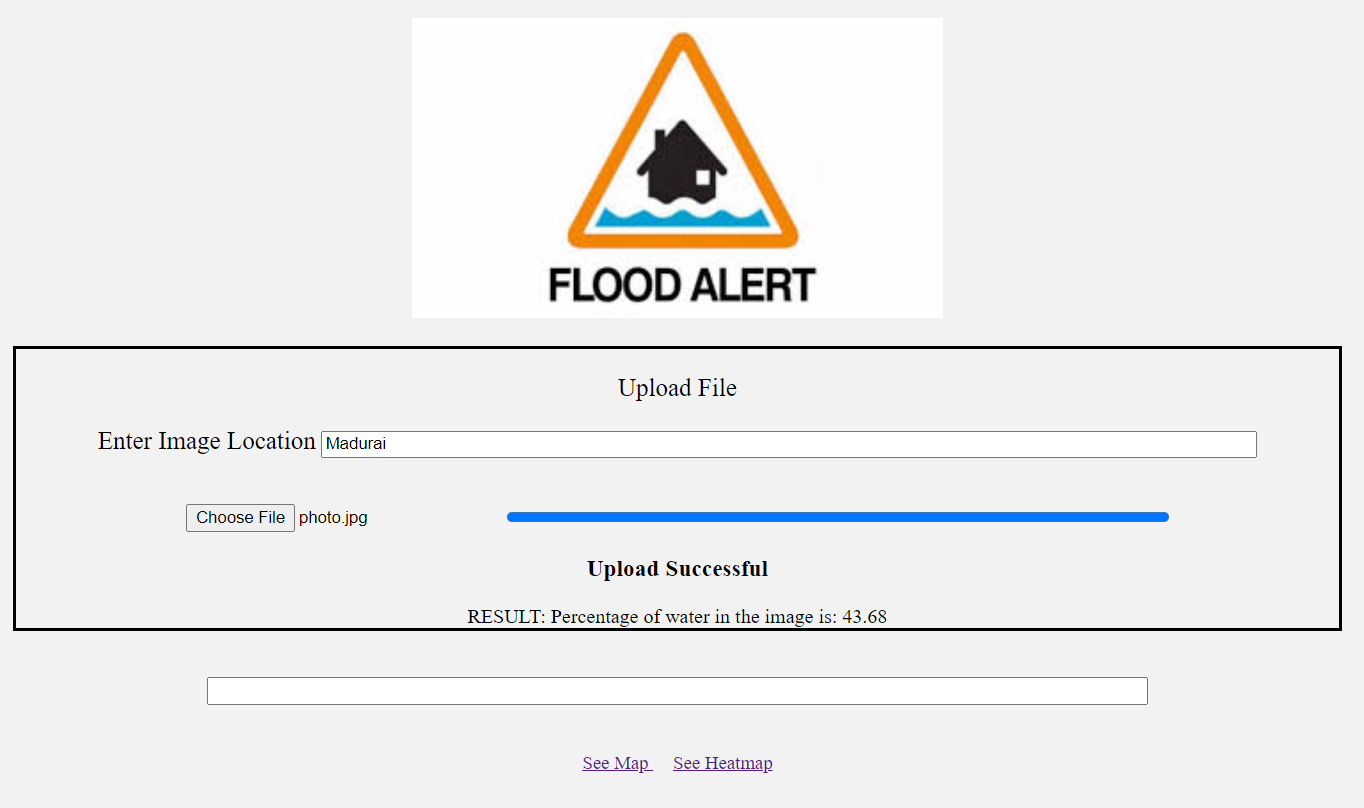
\includegraphics[width=3in]{Capture_upload.png}
		\end{center}
	\caption{Image uploaded undergoing authentication}
	\end{figure}
\subsubsection{Analytics}
The application enables the user to view the clusters of affected zones in his/her city and thus avoid travel there. The heatmap of affected regions is available to the general users to understand the severity or intensity of the catastrophe. \\
One would also be able to quickly glance through the names of the zones or districts severely afflicted. This quick flow of verified information would serve as a boon to the oblivious citizens.
\subsubsection{Mapping peripheries}
With the help of such a quick and responsive application local authorities can use it to their advantage and cordon of these “hotspots” and debar the public from venturing into the area.\\
Delineation of flood risk hotspots is a very challenging task for the authorities which we have automated. The detailed boundary can be used as a reference by civic authorities, power department, municipal corporation, and other local authorities that need to provide urgent relief aid to the affected people.\\
It is important to underline the delineation carried out cannot replace a comprehensive evaluation by experts.
\subsubsection{Usefulness}
This application can be used by the National Disaster Relief Force (NDRF) and other rescue personnel for early detection of flood affected areas and providing urgent relief aids to the affected.\\
After the application is fully deployed, the data it gathers over a period of time can be analyzed to ascertain potential flood prone areas. Mapping the regions requiring robust infrastructure, road maintenance, location of stormwater pumping stations and water tank facilities would become a tad easier for the municipal corporation. \\
The ease of use, responsive nature and prompt flow of real time information directly from the men on the ground providing relief work and subsequent analysis of the data for visualization makes the application unique and highly beneficial. 
\section{System design}
	
\begin{center}
\begin{figure}[h!]
  
    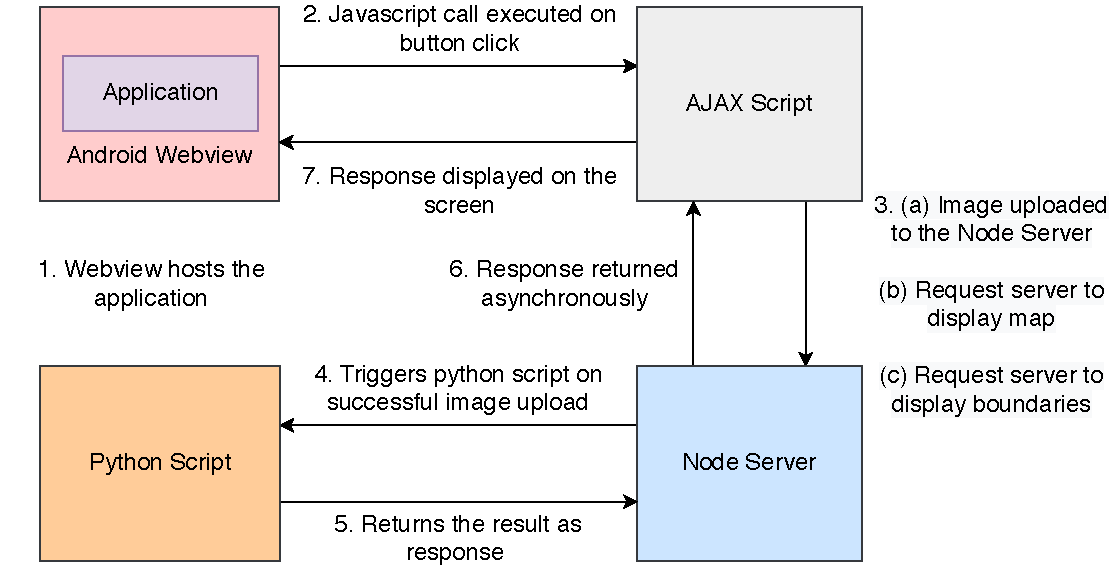
\includegraphics[page=1,width=0.5\textwidth]{System Design.pdf}\hspace*{5\textwidth}
  \caption{Flowchart}
\end{figure}
\end{center}
\subsection{Framework}
	\begin{itemize}
	\item Android webview hosts the html form.
	\item Javascript call executed on button click.
	\item Server script spawns a child process.
	\item Python code executed in the backend.
	\item Backend code accesses the server database.
	\item Returns the required data in JSON format.	
	\end{itemize}
\subsection{Multiple requests}
Node.js runs in a single thread. However, we can take advantage of multiple processes. The spawn method spawns an external application in a new process and returns a streaming interface for I/O. We can pass arguments to the command executed by the spawn as an array using its second argument. In this way, we can send the data from the server to the client side script.\\
In our code, we passed the executable python file as an argument to the spawn method which runs in the backend and provides the output.
\begin{center}
\begin{figure}
  
    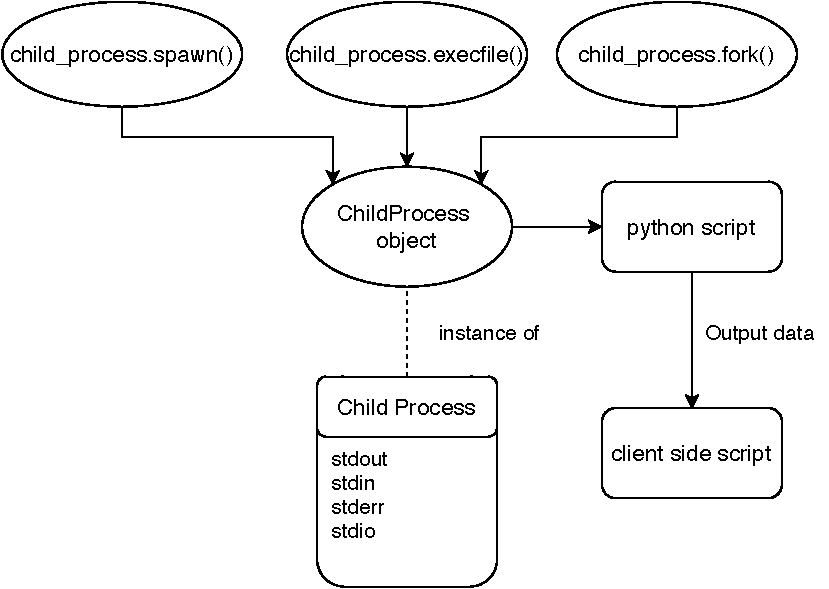
\includegraphics[page=1,width=.47\textwidth]{capture_spawn.pdf}\hspace*{5\textwidth}
  \caption{Handling multiple requests}
\end{figure}
\end{center}
\section{Implementation}
The android app has been prepared using Android Studio. Nodejs Server is used for storing the data and running the script for the detection of flood images.
\subsection{Frontend}

Key features of the flood alert application:
\begin{itemize}
	\item Takes images of affected locations from relief workers.
	\item Authenticates and filters flood images using an AI model.	
	\item Detects the clusters and hotspots that have suffered havoc by the floods
	\item Maps the periphery of the areas that should be avoided by the people and which needs relief aid by NDRF and civic volunteers
\end{itemize}

\subsection{Backend}
The Express Server is used as the Backend module framework. Once the image file reaches the server endpoint, a child process is spawned from the Node Server and a python script is invoked from it. The Python script performs image binarization on the uploaded image and returns the desired output to the Node Server which in turn is sent back as a response to the client and displayed on the screen.
\subsection{Deep learning approach}
The implementation of the backend code is done in python. There are two python scripts:
	\begin{enumerate}
		\item For training using the available datasets.
		\item Prediction of images provided by rescue personnel.
	\end{enumerate}
\subsubsection{Training dataset}
	\begin{enumerate}
	\item \textbf {Generation of flood-water training samples:} To generate training samples of flood-water, we scrapped images from google by typing keywords such as "Mumbai Flood", "Orissa Floods", etc.
Then we manually cropped only the floodwater regions, those were used further for training samples generation. 
\item \textbf {Generation of non-water training samples:} To generate non-water samples, various random keywords were used to gather images from the internet which were not associated with floodwater, a few of them being: animals, house, text, trees, man, volcano, etc.
	\end{enumerate}
	\begin{figure}[h!]
		\begin{center}
		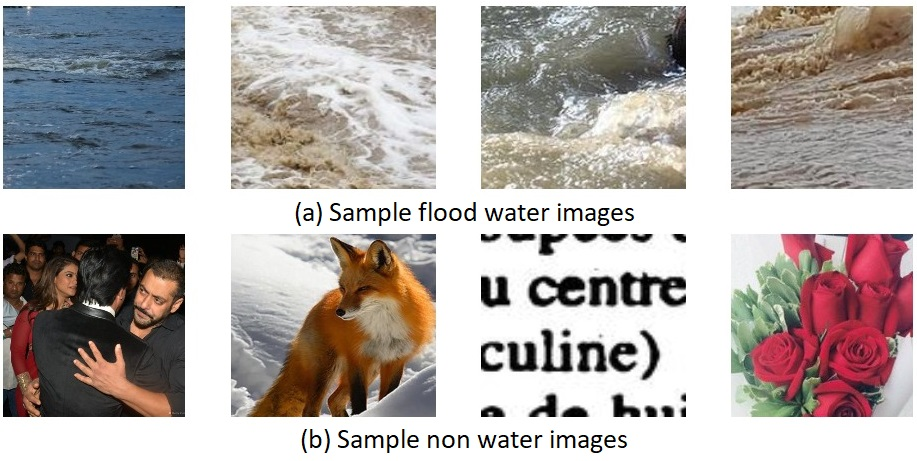
\includegraphics[width=3in]{training_data.jpg}
		\end{center}
	\caption{Sample training data}
	\end{figure}

\subsubsection{Flood-water-detector model}
Convolutional neural networks are a class of deep, feed-forward artificial neural networks. It uses three basic ideas: local receptive fields, shared weights, and pooling. CNN's are translational invariant. In this work, we propose a CNN-based flood-water-detector model.\\
The proposed CNN model is trained using two different kinds of image samples: {(i) flood-water and (ii) non-water}\\
 We use a training sample dimension of $48*48*3$. We run a non overlapping window of size $48*48*3$ over the entire set of images ( both water and non-water) and thus create a dataset of images of size $48*48*3$ The window size $48*48*3$ is moved from left to right and top to bottom, and the image under the window is cropped to produce several image patches.  A total of 54K samples are generated out of flood-water samples and non-water samples. Out of these 50K samples we use 21K samples for training the model and 9K samples are used for the validation of the CNN model. The rest 20K samples are kept for testing the flood-water-detector . \\
We use 2 approaches to create the model:
	\begin{enumerate}
	\item Creating our own model for training and prediction.
	\item Using transfer learning and performing layer unfreezing.
	\end{enumerate}
The training of the models was done on the following
hardware specifications: Intel i5 1.60 GHz, 8 GB RAM and NVIDIA GeForce 940MX 2 GB GPU.
\begin{enumerate}
\item \textbf {The architecture of our own model:}	
The CNN architecture that we used consists of four convolution layers, two fully connected layers (FC), and one softmax layer. Each convolution layer is followed by a dropout layer which is again followed by a rectification layer (ReLU). The output is fed into the max pooling layer which again is fed into the next block of layers. The softmax layer is required for classification. The details of the layers are summarized in Table I.
\begin{table}[h!]
\caption{Architecture of own model}
\resizebox{.5\textwidth}{!}{
	\begin{tabular}{|c|c|c|c|c|}
	\hline
	Serial & Layer & Filter & No. of & Output \\ 
	No. & Type & Dimension & Filters & Dimension \\ \hline
	1 & Input & - & - & $48*48*3$ \\ \hline
	2 & Conv+Dropout(0.2)& $3*3*3$ & 64 & $48*48*64$ \\
	3 & Max Pooling& $2*2$ & - & $24*24*64$ \\ \hline 
	4 & Conv+Dropout(0.2)& $3*3*3$ & 128 & $24*24*128$ \\
	5 & Max Pooling& $2*2$ & - & $12*12*128$ \\ \hline 
	6 & Conv+Dropout(0.2)& $3*3*3$ & 256 & $12*12*256$ \\
	7 & Max Pooling& $2*2$ & - & $6*6*256$ \\ \hline 
	8 & Conv+Dropout(0.2)& $3*3*3$ & 512 & $6*6*512$ \\
	9 & Max Pooling& $2*2$ & - & $3*3*512$ \\ \hline 
	10 & Fully Connected(64) & - & - & $1*1*64$ \\ 
		& Dropout(0.2) & & & \\	
\hline
	11 & Fully Connected (2) & - & - & $1*1*2$ \\
	12 & Softmax (Output) & - & - & $1*1*2$ \\ \hline
	\end{tabular}}
	\end{table}

Total params: 4,980,482 (All Trainable) \\
 Accuracy: 88.23\%\\

\item \textbf {Transfer learning approach:}
With transfer learning, instead of starting the learning process from scratch, we start from patterns that have been learned when solving a different problem.\\
In our problem, we use the VGG19 pretrained model.\\
In VGG19, the image input size is $224*224*3$. However, as discussed earlier, the model is presented with an input image of size $48*48*3$. This is made possible because in transfer learning only the layer weights (i.e the parameters) are loaded which are independent of the size of the input image. \\
Finally, the model has to be fine-tuned according to one of the three strategies:\\
There are 3 ways of using transfer learning:
\begin{enumerate}
\item Freezing the entire convolutional base.
\item Train some layers and leave the others frozen.
\item Use the architecture of the pre-trained model and train it according to our dataset.
\end{enumerate}
All these 3 methods were experimented with. We found out that freezing some layers while unfreezing others performed best as compared to other methods.
The model that performed the best had first 4 blocks of convolution layers frozen while the last convolution block (having 4 convolution layers) unfrozen.\\
Total params: 20,090,306\\
Trainable params: 9,505,154\\
\begin{table}[h!]
\caption{Model Test}
\begin{center}
	\begin{tabular}{|c|c|c|c|}
\hline
Class Label & Precision & Recall & F - score\\ \hline
0 (Non water) & 0.99  & 0.99 & 0.99\\ \hline
1 (water) & 0.91 & 0.89 & 0.90\\ \hline
	\end{tabular}
\end{center}
\end{table}
Accuracy: 97.7\%

\end{enumerate}
Thus, observing the results of both the models we concluded that the model created by the transfer learning approach worked better than our own model. We used the former in our application.
\subsubsection{Response matrix generation (heatmap) and flood region identification}
	\begin{enumerate}
\item 	Response matrix generation: We use an overlapping sliding window approach to generate the response matrix for the input image. The size of the window is $48*48$ and its stride is 8 pixels (both vertical and horizontal). As a preprocessing step, the input image is zero-padded in all the sides of the images. 48 zeros are padded on the four sides of the image under test. These padded elements are discarded later to obtain the final response matrix.\\
Steps for Response Matrix Generation:
		\begin{enumerate}
		\item A Matrix named mask is prepared of the same dimensions of the input image (only 1 channel) $(48*48*1)$
		\item Each image patch $(48*48*3)$ is fed to the flood-water-detector model. The output is a prediction of value 1 (water) or 0 (non-water).
		\item This value is added to all $48*48$  cells in the response matrix mask.
		\end{enumerate}
Algorithm:\\
\begin{equation}
\begin{aligned}
	mask[y:y + winW, x:x + winH] =\\
	 mask[y:y + winW, x:x + winH]+\\
	 np.full((48,48), y\_pred)
\end{aligned}
\end{equation}

where,\\
$winW = winH =48$\\
	\begin{equation}
	y\_pred =
		\begin{cases}
      	0, & \text{if}\ image patch = non water \\
      	1, & \text{if}\ image patch = water \\
    	\end{cases}
	\end{equation}
\item Flood region identification: First the response matrix is divided by the maximum value in the response matrix. Then we convert the value in the matrix mask to 0 or 255 depending upon a threshold:\\
$\displaystyle{mask[i,j]=\frac{mask[i,j]}{maxval}}$
	\begin{equation}
	img[i,j] =
		\begin{cases}
      	0, & \text{if}\ mask[i,j] <= T \\
      	1, & \text{if}\ mask[i,j] > T\\
    	\end{cases}
	\end{equation}
where,
$T \rightarrow Threshold$\\
$0<T<1$\\
maxval $\rightarrow$ Maximum value present in the matrix mask
		
	\begin{figure}[h!]	
		\begin{center}
		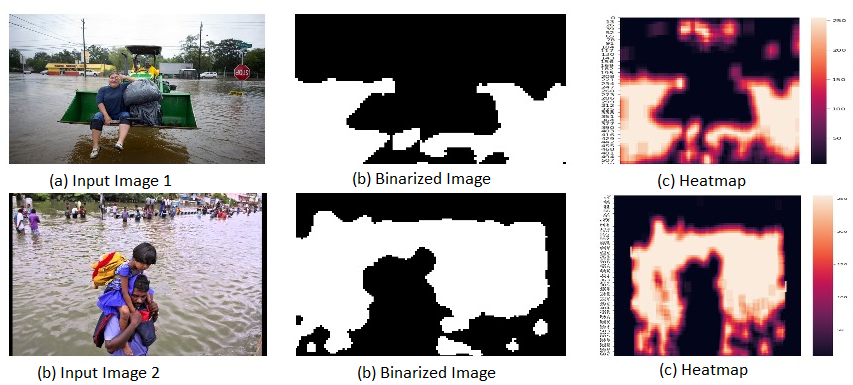
\includegraphics[width=3in]{images.png}
		\end{center}
	\caption{Illustration of floodwater detection}
	\end{figure}
We also used the Otsu Algorithm for the image binarization.
The algorithm divides the image histogram into two classes, by using a threshold such that the in-class variability is very small.\\
Formally, a function g(x, y) can be defined over every pixel value of the original image f(x, y) that defines the new threshold image.\\
	\begin{equation}
	g(x, y)  =
		\begin{cases}
      	0, & \text{if}\ x<T \\
      	1, & \text{if}\ x \geq T \\
    	\end{cases}
	\end{equation}
where,
$T \rightarrow Threshold$\\
\item The region covered by water: After the image binarization, the percentage of the image covered by water is calculated as follows:\\
\begin{equation}
\displaystyle{
\begin{aligned}
	\text{Percentage of the image covered by water} = \\ \frac{\text{No. of water pixel}}{\text{Total no. of pixels}}*100
\end{aligned}}
\end{equation}
\end{enumerate}
The flowchart shown in figure 6 depicts the entire course of actions undertaken to successfully carry out the image binarization task.
\begin{center}
\begin{figure}
  
    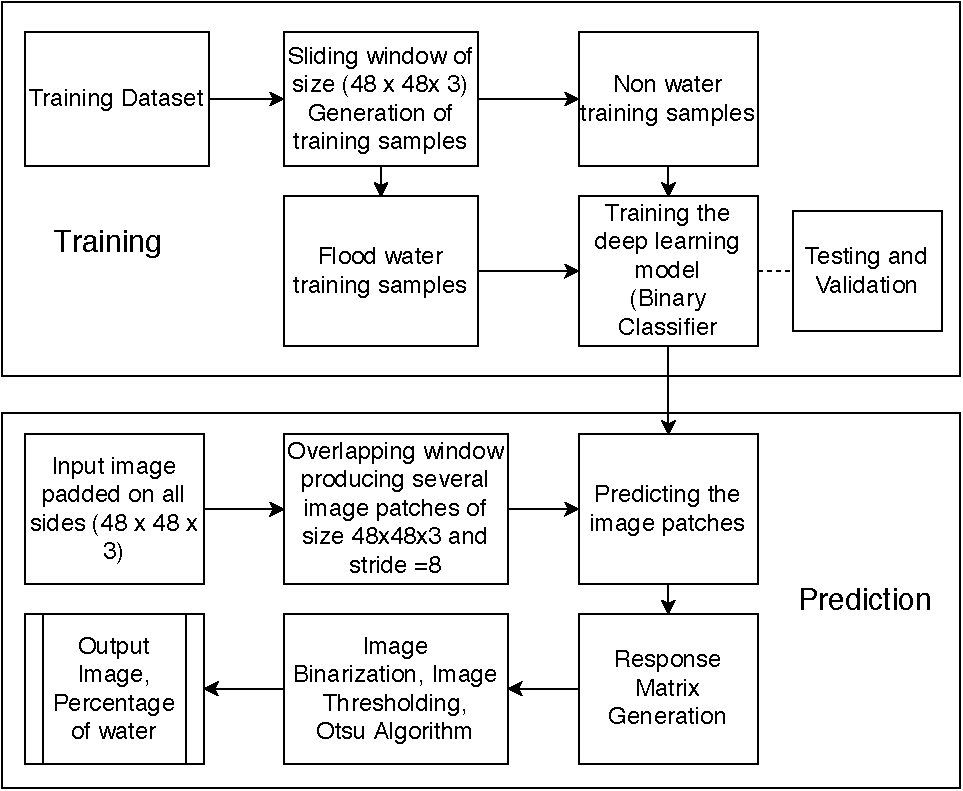
\includegraphics[page=1,width=0.5\textwidth]{flowchart.pdf}\hspace*{5\textwidth}
  \caption{Flowchart}
\end{figure}
\end{center}
\section{Simulation}
In the absence of a real dataset (images from flood-affected locations) we simulated the data by scraping images of major flood havocs in recent years in cities such as Mumbai, Chennai, etc.\\
We scrapped hundreds of images from google using the Selenium web driver and BeautifulSoup python library for pulling data out of HTML and XML files.
\subsection{Assigning coordinates to scrapped images}
Images scrapped from google do not contain geolocations i.e latitude and longitude (location) of the image. Thus to simulate a real calamity scenario (flood) we needed to tweak the metadata of the images and assigned them coordinates.
\\\textbf{Algorithm for selecting coordinates:}\\
We identified certain regions in cities that are low lying areas or are prone to floods. For example, in Mumbai, the areas of Andheri, Kurla, Sion, Juhu, Santacruz, etc were identified.\\
Coordinates of these locations were taken as cluster centers.
Each cluster center is assigned a scrapped image and other images are distributed randomly to each of the clusters. Each cluster has a certain lower limit of the number of images and an upper limit. 
Coordinates for the images were assigned randomly within a 2km radius of the cluster center. This algorithm is just for a simulated scenario and is based on ideal conditions\\
Algorithm for a particular cluster:\\
$\text{cluster\_size=random.randrange(10,150,1)}$ \\
$\text{where, Lower limit =10, Upper limit=150}$\\
$\text{covariance} = $
$\begin{bmatrix}
1 & 0\\
0 & 1\\ 
\end{bmatrix}$
\begin{equation}
\begin{aligned}
x,y = \text{random.multivariate\_normal(cluster\_center,}\\
      \text{covariance,cluster\_size)}
\end{aligned}
\end{equation}
\begin{equation}
\begin{split}
\text{img\_coodinates=cluster\_center} -
\begin{bmatrix}
(2km) & (2km)
\end{bmatrix} +  \\ (
\begin{bmatrix}
4Km 
\end{bmatrix} *
\begin{bmatrix}
x & y 
\end{bmatrix}  )\\
\end{split}
\end{equation}
where, 4 km is the diameter, 
$img\_coordinates$ are the newly assigned coordinates to scrapped images.
\section{Working with the simulated scenario}
After scraping the images, all the images which have floodwater content less than a specified threshold are removed. The deep learning model is used to calculate the  water percentage which has been explained previously in detail. Each marker created in the map for an image has an on click event which opens the image in an infobox and its details.\\
	\begin{figure}[h!]	
		\begin{center}
		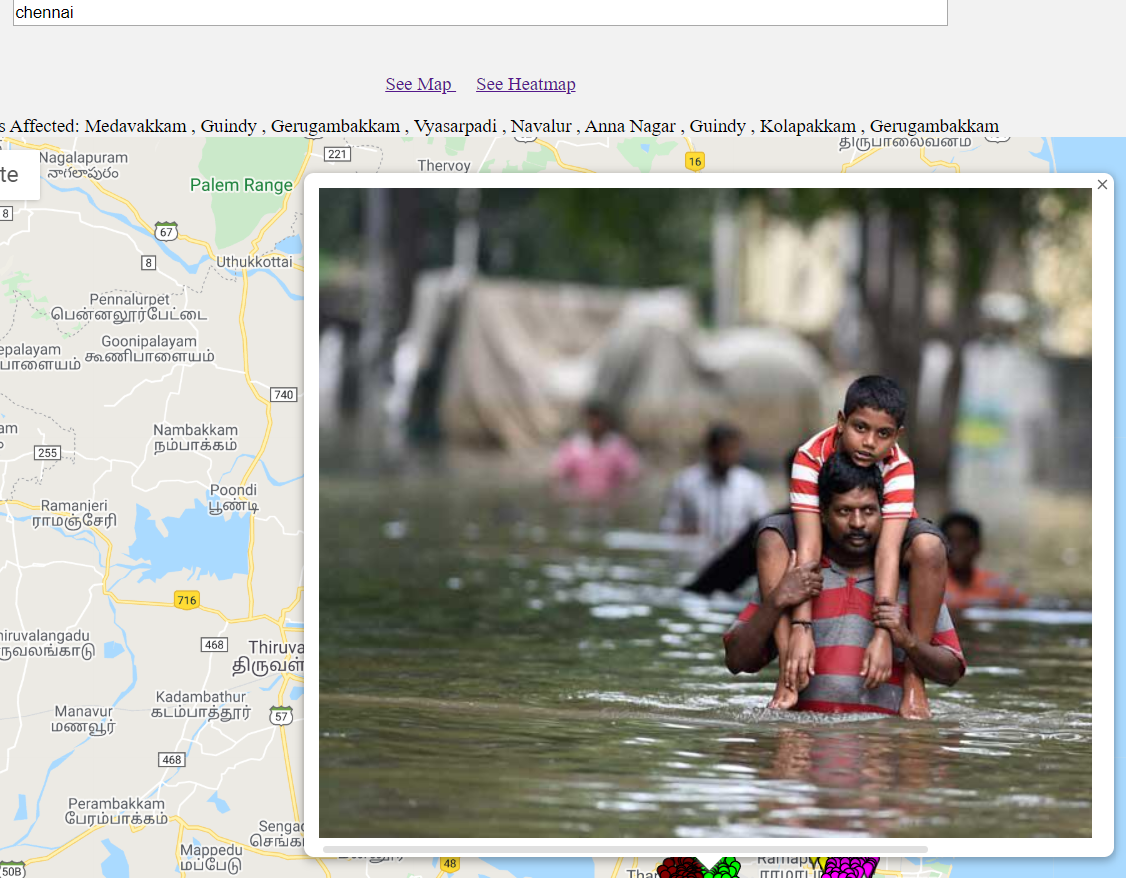
\includegraphics[width=3in,height=1.6in]{Capture_infobox.png}
		\end{center}
	\caption{Image shown in infobox}
	\end{figure}
\subsection{Clustering}
The number of cluster centers is not specified. Thus the most suitable algorithm for clustering when the number of cluster centers and the shape of the cluster is not known is the \textbf{DBSCAN algorithm}.\\
In our application where we have worked with geo-coordinates, the parameters used for the DBSCAN algorithm are as follows:\\
Distance measure = "Haversine"\\
Epsilon = 2 (km) / R, where R = 6373 km is the radius of earth and min\_samples = 5\\
The algorithm used for DBSCAN is the ‘ball tree’. This algorithm can avoid the need to calculate every possible distance. This is because the ball tree algorithm can use the triangular inequality theorem to reduce the number of candidates that need to be checked to find the nearest neighbours of a data point.\\
The DBSCAN algorithm gives the total number of estimated clusters. Using this we further implemented the \textbf{k - means algorithm} which gives the cluster centers.
	\begin{figure}[h!]	
		\begin{center}
		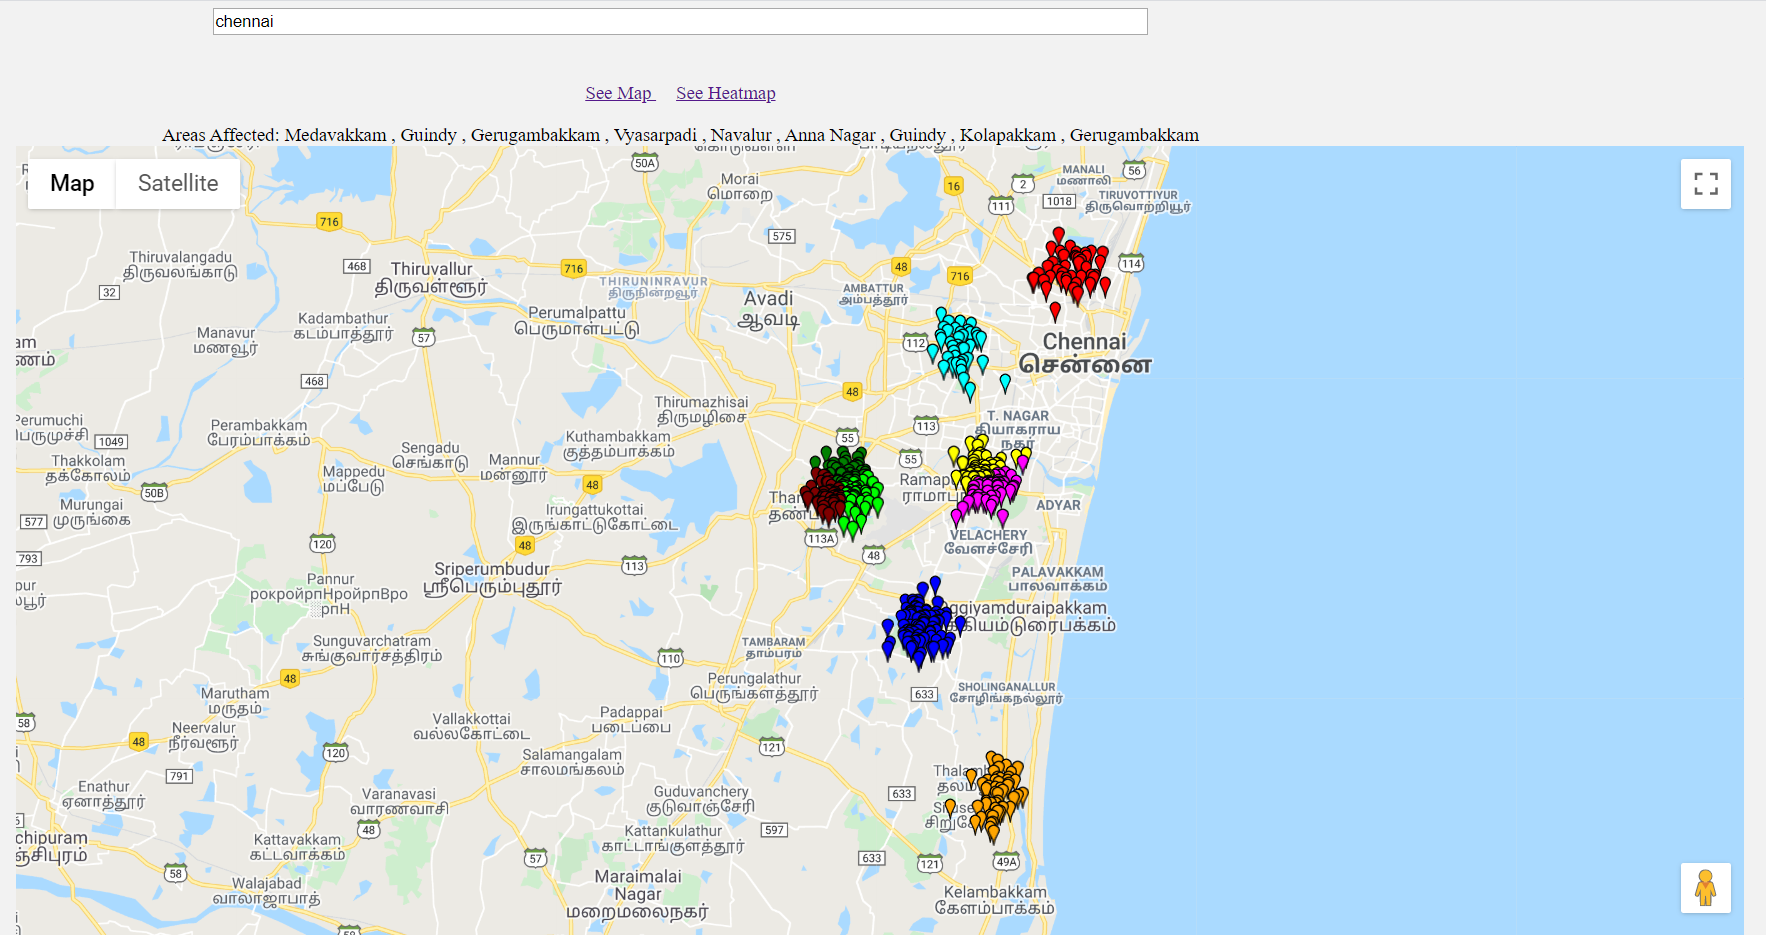
\includegraphics[width=3in,height=1.6in]{Capture_chennai_cluster.png}
		\end{center}
	\caption{Various clusters of regions affected}
	\end{figure}	

\subsection{Generating heatmap}
A heatmap is a visualization used to depict the intensity of data at geographical points. When the Heatmap Layer is enabled, a colored overlay will appear on top of the map. By default, areas of higher intensity will be colored red, and areas of lower intensity will appear green.\\
Heatmap layer has been implemented in our project using the \textbf{google.maps.visualization} library provided by google maps. Various heatmaps are shown in figure 9.
	\begin{figure}[h!]	
		\begin{center}
		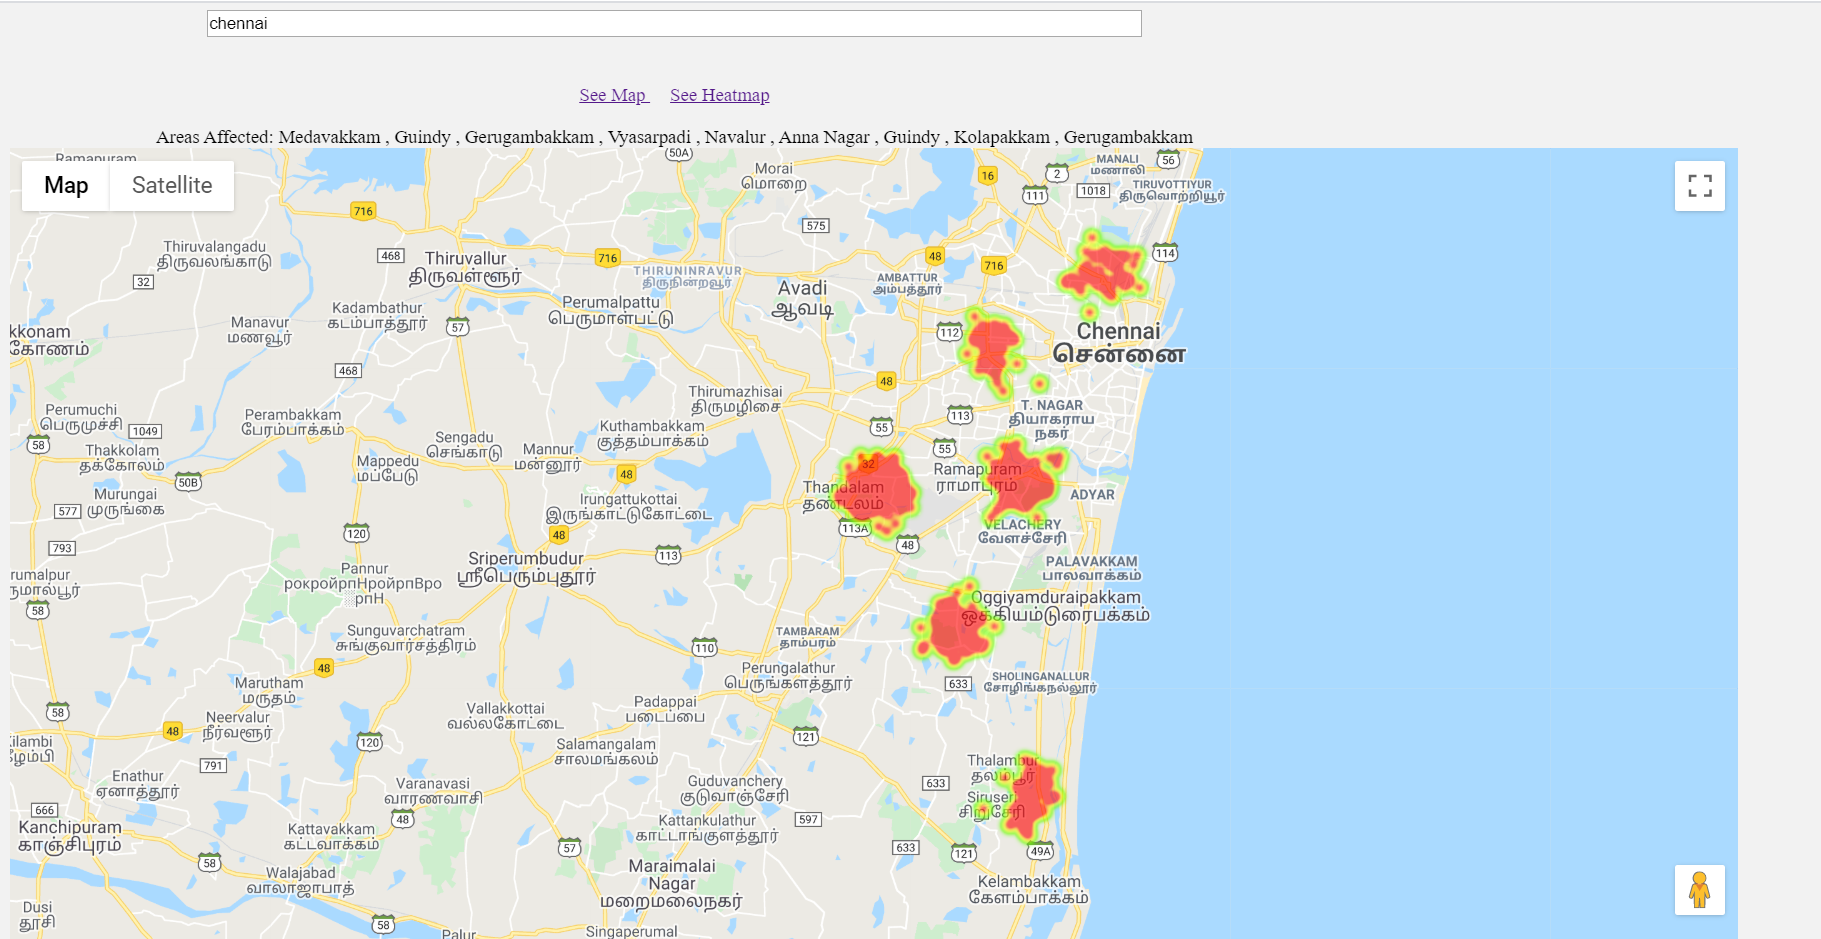
\includegraphics[width=3in,height=1.6in]{Capture_chennai_heatmap_less_boundary.png}
		\end{center}
	\label{fig:Capture_chennai_heatmap_less_boundary}
	\caption{Heatmap layer}
	\end{figure}
	
\subsection{Identifying affected localities}
Coordinates of the cluster centers can be retrieved after applying the k - means clustering on the set of images. These coordinates are helpful to find the center of the affected regions.\\
The set of cluster center coordinates are sent to the ‘The Geocoding API’ in order to get the address of the location.
In this way, we can retrieve the names of localities affected severely by floods.\\
	\begin{figure}[h!]	
		\begin{center}
		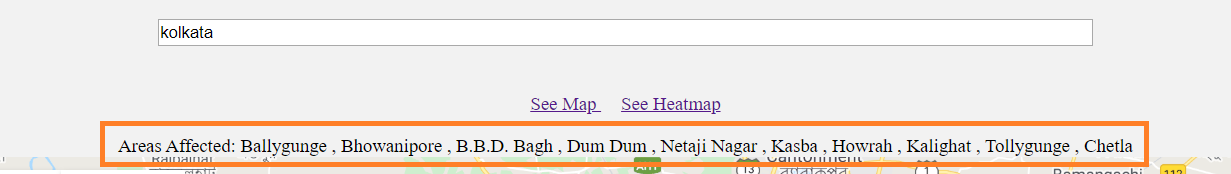
\includegraphics[width=3in]{Capture_kolkata_areas_affected.png}
		\end{center}
	\caption{Areas affected}
	\end{figure}
\subsection{Generating boundaries to identify “hotspots”}
By generating boundaries to the existing clusters of affected regions we can define certain regions as \textbf{“hotspots”} which can be immediately cordoned off to allow only rescue personnel, volunteers, and health workers to access the area and provide relief support to the gravely affected residents of the area. Boundaries are created with the Graham Scan algorithm which creates the smallest polygon encompassing all the coordinates.\\
\textbf{Convex hull}: For a given set of points S, the convex hull, denoted as CH(S), is the intersection of all convex regions containing S. Graham scan algorithm is used to find the convex hull of a set of points.
\begin{algorithm}[h!]
\caption{Graham scan algorithm}
\begin{algorithmic}[1]
\State $ i \gets 2 $ , $ j \gets 3 $ , $ k \gets 4 $
\While {$ k \leq n $}
\If {$P_iP_jP_k \text{ is a right turn}$}
\While {$P_iP_jP_k \text{ is a right turn}$}
\State $\text{Remove edges } P_iP_j \text{ and } P_jP_k $
\State $\text{Add edge } P_iP_k$
\State $j = k$ , $k = k + 1$
\EndWhile
\Else 
\State $\text{ Add edge }P_jP_k \text{ as hull edge}$
\State $i = j$ , $j = k$ , $k = k + 1$
\EndIf
\EndWhile
\end{algorithmic}
\end{algorithm}
where, n is the number of input points.\\
The algorithm takes O(nLogn) time if we use an O(nLogn) sorting algorithm.\\

		\begin{figure}[h!]	
		\begin{center}
		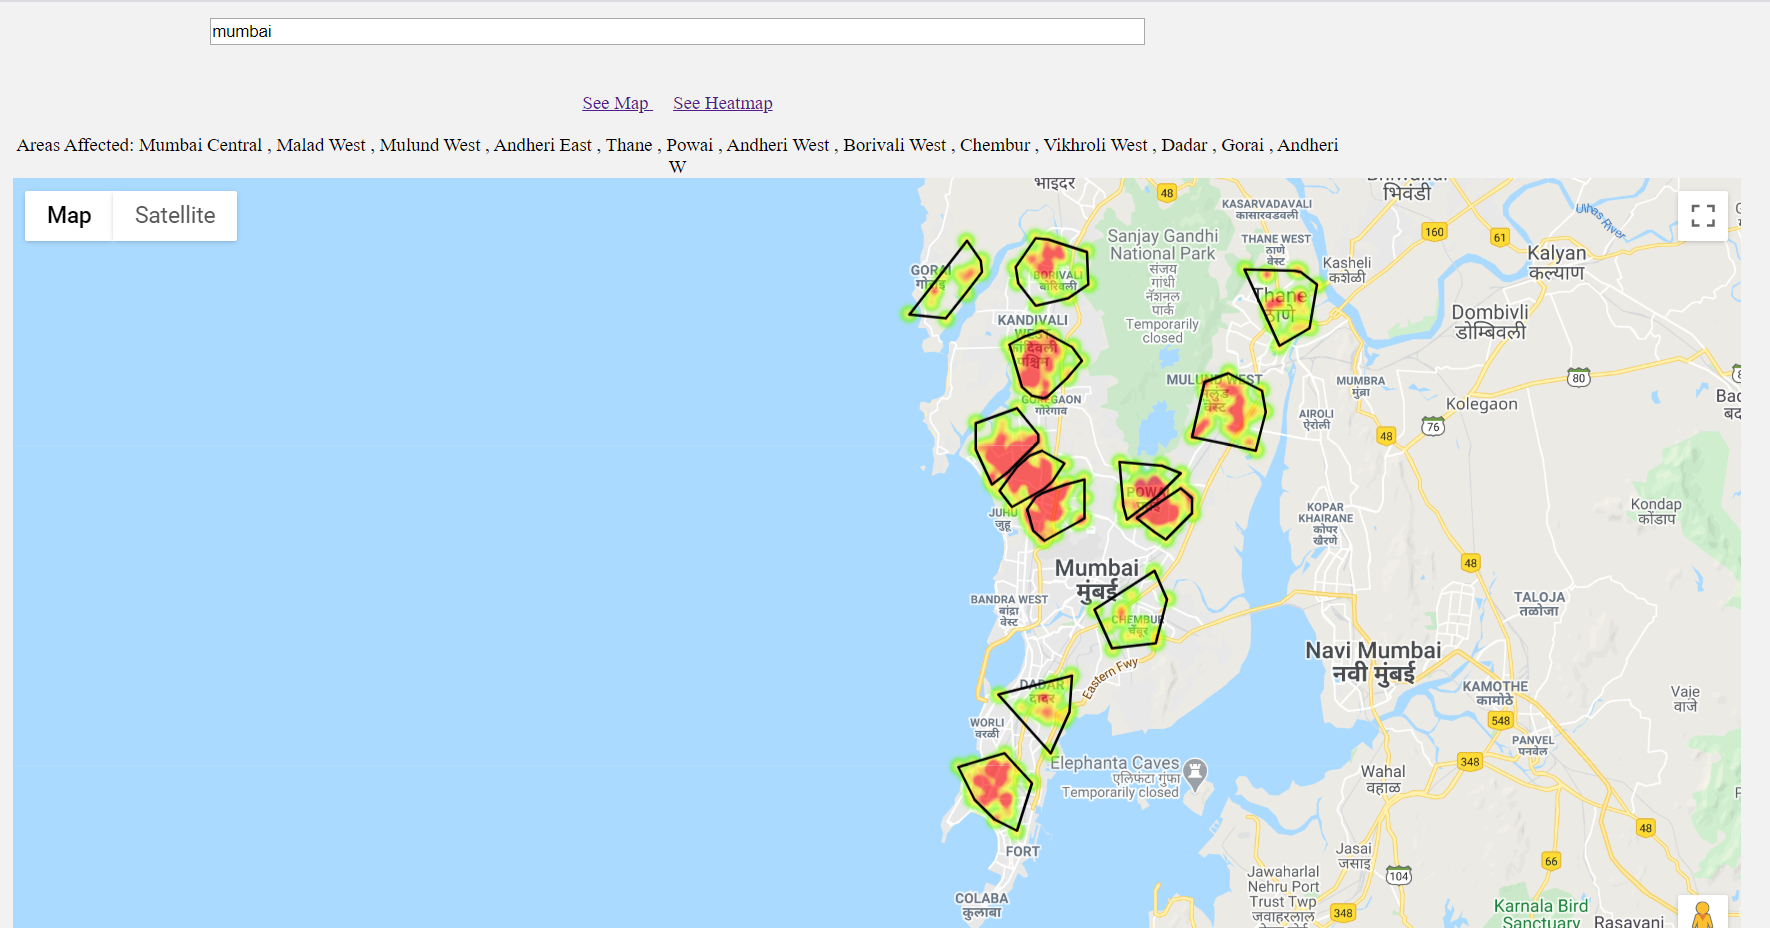
\includegraphics[width=3in]{Capture_mumbai_heatmap.png}
		\end{center}
	\caption{Generating heatmap and identifying hotspots}
	\end{figure}
\section{Results}
\begin{enumerate}
\item The model developed is very accurate (~95\%) in detecting water and non-water regions in the image.
\item The overlapped sliding window approach helps in effectively binarizing the image into water and non-water regions.
\item The deep learning approach to calculate the percentage of floodwater in the image effectively filters out unwanted and wrong images that have been uploaded to the application.
\item The images uploaded in the application would be readily available to the public and it would notify the people of regions affected by the calamity.
\item Citizens traveling across the city and public transport can be made cautious to restrain themselves from traveling to such disaster affected regions.
\item The localities identified as "hotspots" would quickly alert the rescue personnel and civic volunteers to carry out relief operations in those zones.
\end{enumerate}
\section{Future scope}
\begin{enumerate}
\item Over a period of time the data can be analyzed and certain flood prone “hotspots” can be identified which need robust infrastructure, road maintenance, and \textbf{stormwater drainage} facilities.
\item The strategic location of emergency shelter homes can be found out.
\item Such data would be very useful for municipal corporations and NDRF teams working during crisis periods.
\end{enumerate}
\section{Challenges}
\begin{enumerate}
\item The results obtained using the deep learning models had very good training accuracy as well as test accuracy. However, it performed moderately in image segmentation. Thus there is a need for performing other image segmentation and preprocessing     techniques and a comparative study between different techniques.
\item Certain portions in the water which have reflections or shadows are treated as non-water objects. There is scope for improvement in this aspect.
\item Only those images having locations in their metadata can be accepted by the application.
\item Deliberately manipulating image metadata and uploading fake images remains a challenge. 
\item To make the application useful, there must be general awareness among the public and eagerness to contribute towards the benefit of society. 
\bibliographystyle{IEEEtran}
\end{enumerate}
%\cite{8882877}
%\cite{8075343}
%\cite{inproceedings}
%\cite{Chaudhary2019FLOODWATERLE}
%\cite{8688775}
%\cite{8282518}
%\cite{8474802}
%\cite{7392736}
%\cite{10.1145/3341105.3374023}
%\cite{8917368}
%\cite{8203586}
%\cite{10.1145/3065386}
\bibliography{References}

\end{document}